
Siin peatükis tuuakse mõned näiteid, kuidas loodud tööriista saab kasutada ühistranspordi analüüsimiseks.

\section{Tulemuste võrdlus muude linnadega}


Tallinna ühistranspordi busside keskmiseks kiiruseks saadi 20 km/h. Trammide kiiruseks saadi 15 km/h ja mõlemat arvestades saadi keskmiseks kiiruseks 19,7 km/h.
Peatükis \ref{section:valideerimine} toodi välja, et kohati on kiirused kuni 5\% aeglasemad tegelikkusest ehk kuni 1 km/h.

Seda arvestades on Tabelis \ref{tab:maailmaKiirused} välja toodud Stockholmiga võrreldes Tallinna bussid 15 - 20\% aeglasemad.
Trammide kiirusi Stockholmis ei vaadeldud, kuid ülejäänud Euroopaga võrreldes on trammid kuskil 10\% aeglasemad. Seevastu Riiaga võrreldes on ühistransport sama kiire. Tundub, et seis ei ole kõige hullem kuid saaks paremini.

\section{Vanasadama tramm ja avalik arvamus} 

1. detsembril 2024 avati Tallinnas uus trammiliin \cite{err_trammiliin_2024}. Kuna endine trammiliin number 2 suunati läbi sadama sõitma, siis huvitas autorit, et kuidas see erineb trammiliin 1 ajakulust (Joonis \ref{fig:Liin1VsLiin2V2}).
 
Joonis \ref{fig:Liin1VsLiin2V2} kuvatud statistika juurest ilmnes, et läbi sadama sõitmine on aeglasem. Nimelt kulus trammiliinil 1 keskmiselt 4,5 minutit ja trammiliinil 2 keskmiselt 7 minutit kahe punkti vahel liikumiseks. See tähendab, et läbi sadama sõitmine muutis antud sektsioonil trammiliikluse 2,5 minutit aeglasemaks. 

Autor on olnud varasemast grupis nimega "Linnad ja liikuvus", mis on leitav Facebookist. Avalikku gruppi kuuluvad ja seal sõna võtavad näiteks Tallinna abilinnapead Kristjan Järvan, Peeter Pärtel Pere, Madle Lippus ja teised hetkel Tallinna ühistranspordi tulevikku kujundavad isikud.

Laskumata detailidesse nägi autor grupis postitust sadamatrammist  ja seal all kommentaare uue marsruudi rohkest ajakulust (eelnevalt sõitis tramm number 2 mööda mere puiesteed). Toodi välja, et tunnetuslikult olevat läbi sadama minemine kuni 10 minutit aeglasem, kuid puudusid konkreetsed andmeid.

Teades, et tegelikult oli trammiliini 2 teekond 2,5 minutit aeglasem  ei saanud seda mitte märkimata jätta. Joonisel \ref{fig:facebookiPostitus} ongi näha postituse alla tehtud kommentaar, kuhu lisati vastav tekst ja pilt. Autori hinnangul aitas see tuua faktilist tausta ja sellega koos aitas väikestviisi muuta avalikku arvamust. Sellistel väikestel mõjutustel võib pikemas plaanis olla arvestatav mõju ja sellega on ühtlasi ka osaliselt täidetud autori esialgne eesmärk. 
\begin{figure}[h!]
    \centering
    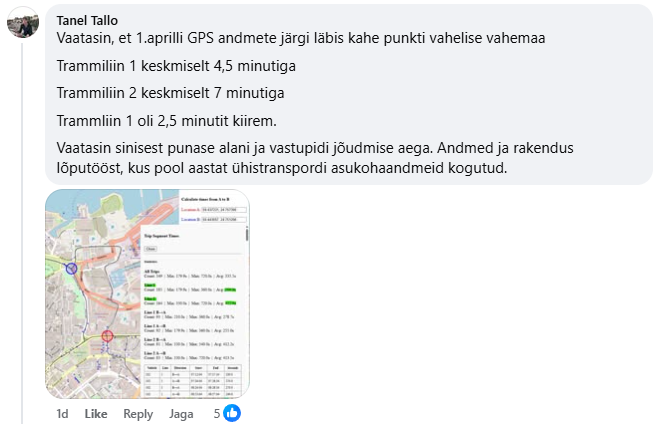
\includegraphics[width=0.8\textwidth]{figures/facebookiPostitus.png}
    \caption{Sotsiaalmeedia postituse kommentaar trammiliini 1 ja 2 võrdlusest.}
    \label{fig:facebookiPostitus}
\end{figure}

\section{Trammiliini 4 graafikus püsimine}

Graafikus püsimise täpsuse uurimiseks kasutati Joonisel \ref{fig:Liin1VsLiin2V2} olevat tööriista ning saadud andmed sisestati Google Spreadsheeti \cite{Spreadsheet}, mille abil saadi Joonis \ref{fig:kalevVaikePaala}.
\begin{figure}[h!]
    \centering
    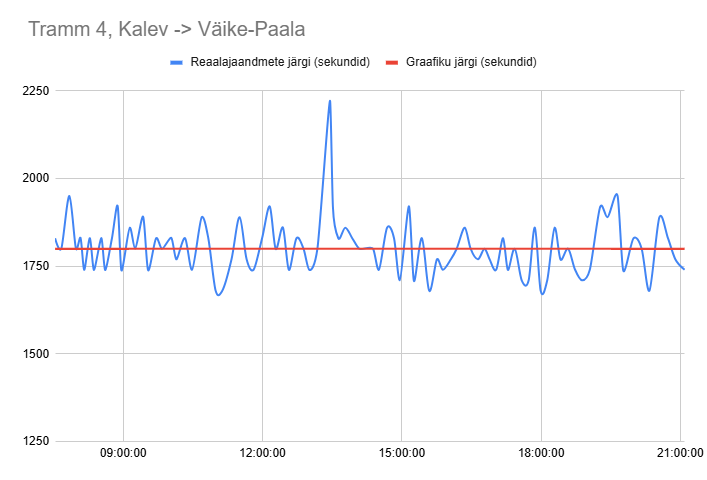
\includegraphics[width=0.85\textwidth]{figures/kalev-vaikepaala-kiirused.png}
    \caption{Graafikus püsimise täpsus.}
    \label{fig:kalevVaikePaala}
\end{figure}
Graafiku järgi kulus kella 07:00 hommikust kuni poole kümneni õhtul alati 30 minutit Kalevist Väike-Paalasse sõitmiseks. Reaalajaandmete järgi kulus keskmiselt 30 minutit ja 4 sekundit. 73\% kordadest jõudis sõiduk kohale kuni 1-minutlise veaga. Ühel korral toimus suurem hilinemine, kus sõidukil kulus 7 minutit. Sõiduk peatus Paberi peatuse juures ligikaudu 5 minutit.

Üldiselt on graafikus püsimise täpsus hea. Päeva lõikes ei ole ka näha, et tipptundidel oleks ajakulu kuidagi suurem.

\section{Bussiliini ja ekspressliini võrdlus}

Bussiliin 83 ja ekspressliin 11 sõidavad sama marsruuti mööda peatuset Keemia peatuseni Estonia. Seetõttu olid need head liinid, mida võrrelda.
\begin{figure}[h!]
    \centering
    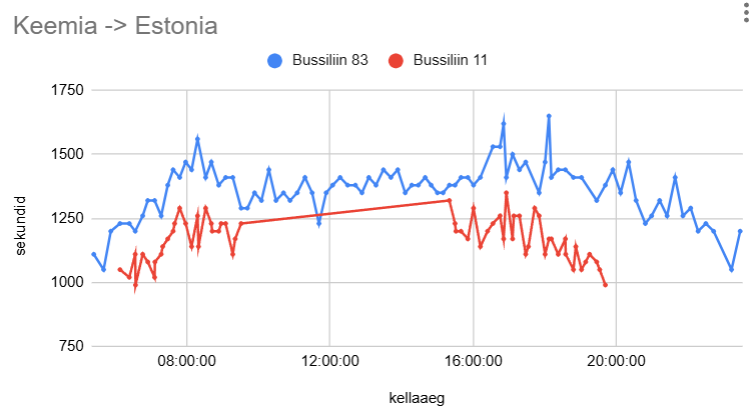
\includegraphics[width=0.8\textwidth]{figures/keemia-estonia.png}
    \caption{Kahe bussiliini ajakulu võrdlus.}
    \label{fig:keemiaEstonia}
\end{figure}

Nagu Jooniselt \ref{fig:keemiaEstonia} näha, siis ekspressliin on kiirem. Kuigi kella viiesel tipptunnil on näha, et vahe ei ole alati väga suur. Kahel korral oli vahe 1 minut ja kahel korral 1,5 minutit. Bussiliini 83 juures on varahommikul ja hilisõhtul  ajakulu märksa väiksem. Liikluse tihenedes muutus see suuremaks. 

Vaadeldes ainult aegu, millal mõlemad sõitsid, siis hommikul oli ekspressliin keskmiselt 3,5 minutit kiirem ja õhtul 4,5 minutit kiirem. Keskmiselt oli ekspressliin 17\% kiirem. Tulemused on mõneti üllatavad, kuna vahe polegi nii suur kui eeldada. Mustamäe osas peatuvad mõlemad liinid suuresti samades peatustes ja võitu eriliselt pole. Kuid, kui vaadelda viimasest Mustamäe peatusest Siili peatuseni Estonia, siis on ekspressliin ligi 30\% kiirem ja ajaliselt keskmiselt 4 minutit.

\section{Teelõigu võrdlus}
Võimalik on ka saada ülevaade tervest teelõigu ajakulust päeva lõikes.
Näiteks uuriti Pärnu maantee Kesklinna jäävat osa.

\begin{figure}[h!]
    \centering
    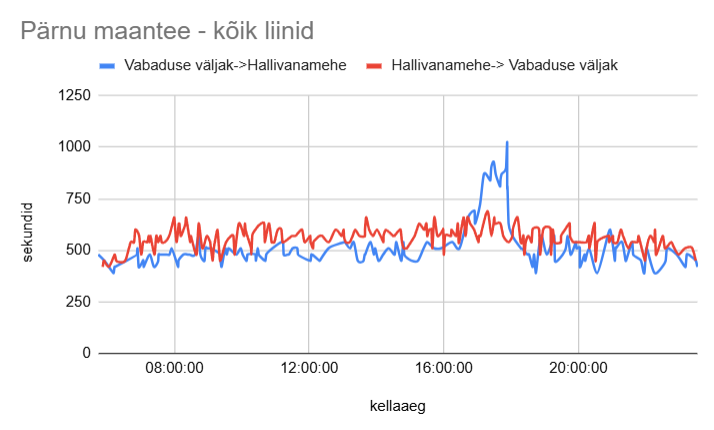
\includegraphics[width=0.9\textwidth]{figures/parnumnt.png}
    \caption{Teelõigu ajakulu väljavõte.}
    \label{fig:parnumnt}
\end{figure}

Nagu Jooniselt \ref{fig:parnumnt} näha, siis päeva jooksul oli suund Vabaduse väljaku poole pidevalt veidi aeglasem, kuid tipptunnil ajakulu ei suurenenud. Seevastu Vabaduse väljaku poolt tulles oli ajakulu suurem 16:30 ja 18:00 vahel. Sel ajaperioodil kulus keskmiselt 5 minutit rohkem kui sellele eelneval ajal. Ajakulu kasvas 8 minuti pealt 13 minuti peale ehk 60\%. 

Kasutaja poolest on ilmselt parem pidevalt ühtlane kiirus, kui tipptunnil  suurem ajakulu. Peatükis \ref{section:Kiirused-kaardil} kirjeldatud tööriista abil vaadeldi, et sisuliselt kogu teekond Pärnu maantee viaduktist kuni Hallivanameheni oli tipptunnil ühissõidukile punane. Täies pikkuses ühissõidukiraja loomine on hetkel ilmselt liiga suur ettevõtmine, kuid kui tuleviks peaks tramm Järve keskuseni sõitma hakkama, siis oleks  antud andmete järgi mõistlik ehituse käigus ka ühisrada planeerida \cite{err_jarve_tramm_2024}.

Kaardirakenduse Waze \cite{waze} järgi võtab autoga Vabaduse väljakult Hallivanameheni jõudmine tipptunnil aega kuskil 10 minutit. Jättes kõrvale bussipeatusesse kõndimise ja sõiduki ootamise, siis bussiraja olemasolul oleks tipptunnil buss antud teekonnal autost tõenäoliselt kiirem.  See võiks muuta Pärnu maanteed mööda liikuvaid ühistranspordiliine atraktiivsemaks. Seeläbi tõuseks Pärnu maantee läbilaskevõime, kuna bussidesse mahub rohkem inimesi.

\section{Edasiarenduste võimalused}

Töö raames loodud lahendused aitavad visualiseerida üldist pilti. Täpsemate tulemuste nägemiseks saaks teha mitmeid edasiarendusi.

Sõidugraafikute integreerimise tulemusena saaks näha, millistel liinidel ja mis peatustes toimub kõige rohkem kõrvalekaldeid. Saaks näha kaua keskmiselt üks sõiduk peatuses peatub ja kas Tallinnas on kohti, kus see on keskmisest oluliselt kõrgem.

Ühe lisana oleks võimalik uurida reaalajaandmete järgi busside kobardumist. See tähendab, kui bussid saabuvad samasse peatusesse samal ajal. Saaks näha, mis peatustes või lõikudel seda kõige rohkem juhtub.

Keskmiste kiiruste arvutamise täpsuse tõstmiseks saaks sobitada sissetulevaid sõidukite asukohti reaalsete liinide peale (\textit{map matching}). See võimaldaks vältida kurvide sirgeksvõtmisest tulenevaid probleeme, kuid võib suurendada probleeme juhul, kui teel oli takistus ja sõiduk pidi minema teist teed pidi. 

Kuigi iga 30 sekundi tagant kogumine tähendas siin töös kiiremaid päringuid, lihtsamat töötlemist ja väiksemat andmebaasi, siis võiks kaaluda tihedamalt kogumist. Näiteks iga 10 sekundi tagant kogumine võiks anda parema täpsuse. Loodud andmebaasi struktuur ja andmed tuleks viia GTFS standardile vastavaks. Selliselt oleks andmebaasi andmeid kolmandatel osapooltel lihtsam kasutada.

Praegu kasutuses olev PostGIS andmebaasi laiend võimaldab küll teha geograafilisi päringuid lihtsasti, kuid sõidukite sõitude analüüsimiseks saaks lisada rohkemate lisadega laiendit nimega MobilityDB \cite{mobilitydb}. See on spetsiaalselt loodud järjestatud geograafiliste aegridade analüüsimiseks. See ei asenda PostGIS laiendit, kuid võimaldaks lisafunktsioone. Näiteks hetkel saab lihtsasti kätte sõiduki läbitud geograafiliste asukohtade jada \cite{postgis}, kuid ilma ajalise mõõtmeta. MobilityDB lahendaks selle mure, kuna võimaldab lisada igale asukohale näiteks kellaaja ja kiiruse. Lisaks, kui praegu on sõiduki asukohaandmed andmebaasis olemas kella 14:30:00 ja  14:30:30 jaoks, siis MobilityDB abil saaks leida eeldatava kiiruse ja asukoha ükskõik millal, ka kell 14:30:15. Päringute puhul ei oleks enam oluline teada konkreetset aega ega asukohta.

